\ifx\boi\undefined\ifx\problemname\undefined
\providecommand\sampleinputname{}
\providecommand\sampleoutputname{}
\documentclass[icelandic]{templates/boi}
\problemlanguage{.is}
\fi
\newcommand{\boi}{Eystrasaltsólympíuleikarnir í forritnu}
\newcommand{\practicesession}{Æfingakeppni}
\newcommand{\contestdates}{27. apríl - 1. maí, 2018}
\newcommand{\dayone}{Dagur 1}
\newcommand{\daytwo}{Dagur 2}
\newcommand{\licensingtext}{This problem is licensed under CC BY-SA 4.0.}
\newcommand{\problem}{Verkefni}
\newcommand{\inputsection}{Inntak}
\newcommand{\outputsection}{Úttak}
\newcommand{\interactivity}{Gagnvirkni}
\newcommand{\grading}{Flokkun}
\newcommand{\scoring}{Stigagjöf}
\newcommand{\constraints}{Takmarkanir}
\renewcommand{\sampleinputname}{Sýnidæmis inntak}
\renewcommand{\sampleoutputname}{Sýnidæmis úttak}
\newcommand{\sampleexplanation}[1]{Útskýring á sýnidæmi #1}
\newcommand{\sampleexplanations}{Útskýringar á sýnidæmum}
\newcommand{\timelimit}{Tímamörk}
\newcommand{\memorylimit}{Minnismörk}
\newcommand{\seconds}{s}
\newcommand{\megabytes}{MB}
\newcommand{\group}{Hópur}
\newcommand{\points}{Stig}
\newcommand{\limitsname}{Takmarkanir}
\newcommand{\additionalconstraints}{Auka takmarkanir}
\newcommand{\testgroups}{
Lausnin þín verður prófuð á einhvern fjölda prufuhópa, hver hópur gefur einhvern fjölda stiga.
Hver hópur inniheldur einhvern fjölda prufutilvika.
Til að fá stig fyrir hóp þarftu að leysa öll prufutilvik innan hópsins.
Lokastigin eru fengin úr skilunum sem gáfu hæst stig.
}
\fi
\def\version{jury-1}
\problemname{Leiðir}
{\em Net} er stærðfræðilegt mynstur sem er samansett af mengi hnúta og mengi leggja, þar sem hver leggur tengir tvo hnúta. Dæmi um net með $4$ hnútum og $3$ leggjum er sýnt í útskýringu sýnidæma að neðan.

{\em Leið} i neti er skilgreint sem raðaður listi af $2$ eða fleiri hnútum, þannig að það sé leggur milli samliggjandi hnúta í listanum.
Í þessu verkefni höfum við aðeins áhuga á {\em einföldum leiðum} þar sem enginn hnútur kemur fyrir oftar en einu sinni. Taktu eftir
að listinn er raðaður, til dæmis, ``\texttt{5-6-7}'', ``\texttt{5-7-6}'' og ``\texttt{7-6-5}'' eru mismunandi leiðir.

%For example, a road map could be a graph, if the vertices are towns or other places and the edges are roads that directly connect two places.

Í þessu verkefni er hver hnútur í netinu litaður með einum a $K$ litum. Verkefnið er að finna fjölda
mögulegra (einfaldra) leiða þar sem engir tveir hnútar eru litaðir eins.

\section*{\inputsection}
Fyrsta línan af inntakinu inniheldur þrjár heiltöllur: $N$ (fjöldi hnúta), $M$ (fjöldi leggja), og $K$ (fjöldi mismunandi lita).

%($1 \le N, M \le 3 \cdot 10^5, 1 \le K \le 5$).

Önnur línan af inntakinu inniheldur $N$ heiltölur á milli $1$ og $K$ -- litirnir á hverjum hnút (byrjar á hnút $1$ og endar á hnút $N$).

Næst koma $M$ línur, hver og ein þeirra lýsir legg og inniheldur tvær heiltölur $a, b$ ($1 \le a, b \le N, a \neq b$) -- hnútarnir tveir eru tengdir með leggnum.
Fyrir hverja tvo hnúta er mesta lagi einn leggur á milli þeirra.

\section*{\outputsection}
Skrifaðu út eina heiltölu -- fjölda leiða þar sem allir hnútarnir hafa mismunandi liti. Þessi tala verður alltaf minni en $10^{18}$.

\section*{\constraints}
\testgroups

\noindent
\begin{tabular}{| l | l | l |}
\hline
\group & \points & \limitsname \\ \hline
1      & 23      & $1 \le N, M \le 100, 1 \le K \le 4$ \\ \hline
2      & 20      & $1 \le N, M \le 300\,000, 1 \le K \le 3$ \\ \hline
3      & 27      & $1 \le N, M \le 300\,000, 1 \le K \le 4$ \\ \hline
4      & 30      & $1 \le N, M \le 100\,000, 1 \le K \le 5$ \\ \hline
\end{tabular}

\section*{\sampleexplanation{1}}

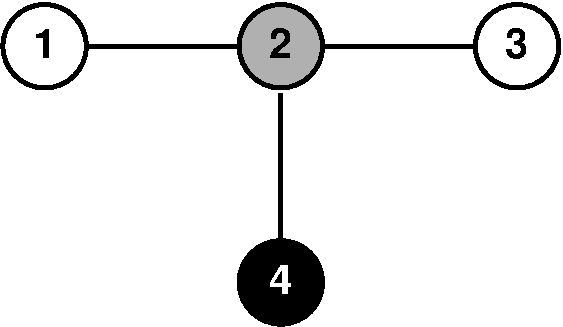
\includegraphics[width=5cm]{pathsfig.pdf}

Netið í fyrsta sýnidæminu er sýnt á myndinni, þar sem hver hnútur hefur verið litaður með hvítum (litur 1) , gráum (litur 2) eða svörtum (litur 3) lit.
Það eru 10 leiðir þar sem allir hnútarnir hafa mismunandi liti: ``\texttt{1-2}'', ``\texttt{2-1}'', ``\texttt{2-3}'', ``\texttt{3-2}'', ``\texttt{2-4}'', ``\texttt{4-2}'', ``\texttt{1-2-4}'', ``\texttt{4-2-1}'', ``\texttt{3-2-4}'' og ``\texttt{4-2-3}''.

Taktu eftir að ``\texttt{1}'' er ekki leyft sem leið, því það er aðeins einn hnútur. 
``\texttt{1-2-3}'' er einnig ekki leyft því það inniheldur tvær nóður með lit $1$.
